\hypertarget{framegen_8h}{
\section{framegen.h File Reference}
\label{framegen_8h}\index{framegen.h@{framegen.h}}
}
The framegenerator for Xilinx FPGA. 



This graph shows which files directly or indirectly include this file:\begin{figure}[H]
\begin{center}
\leavevmode
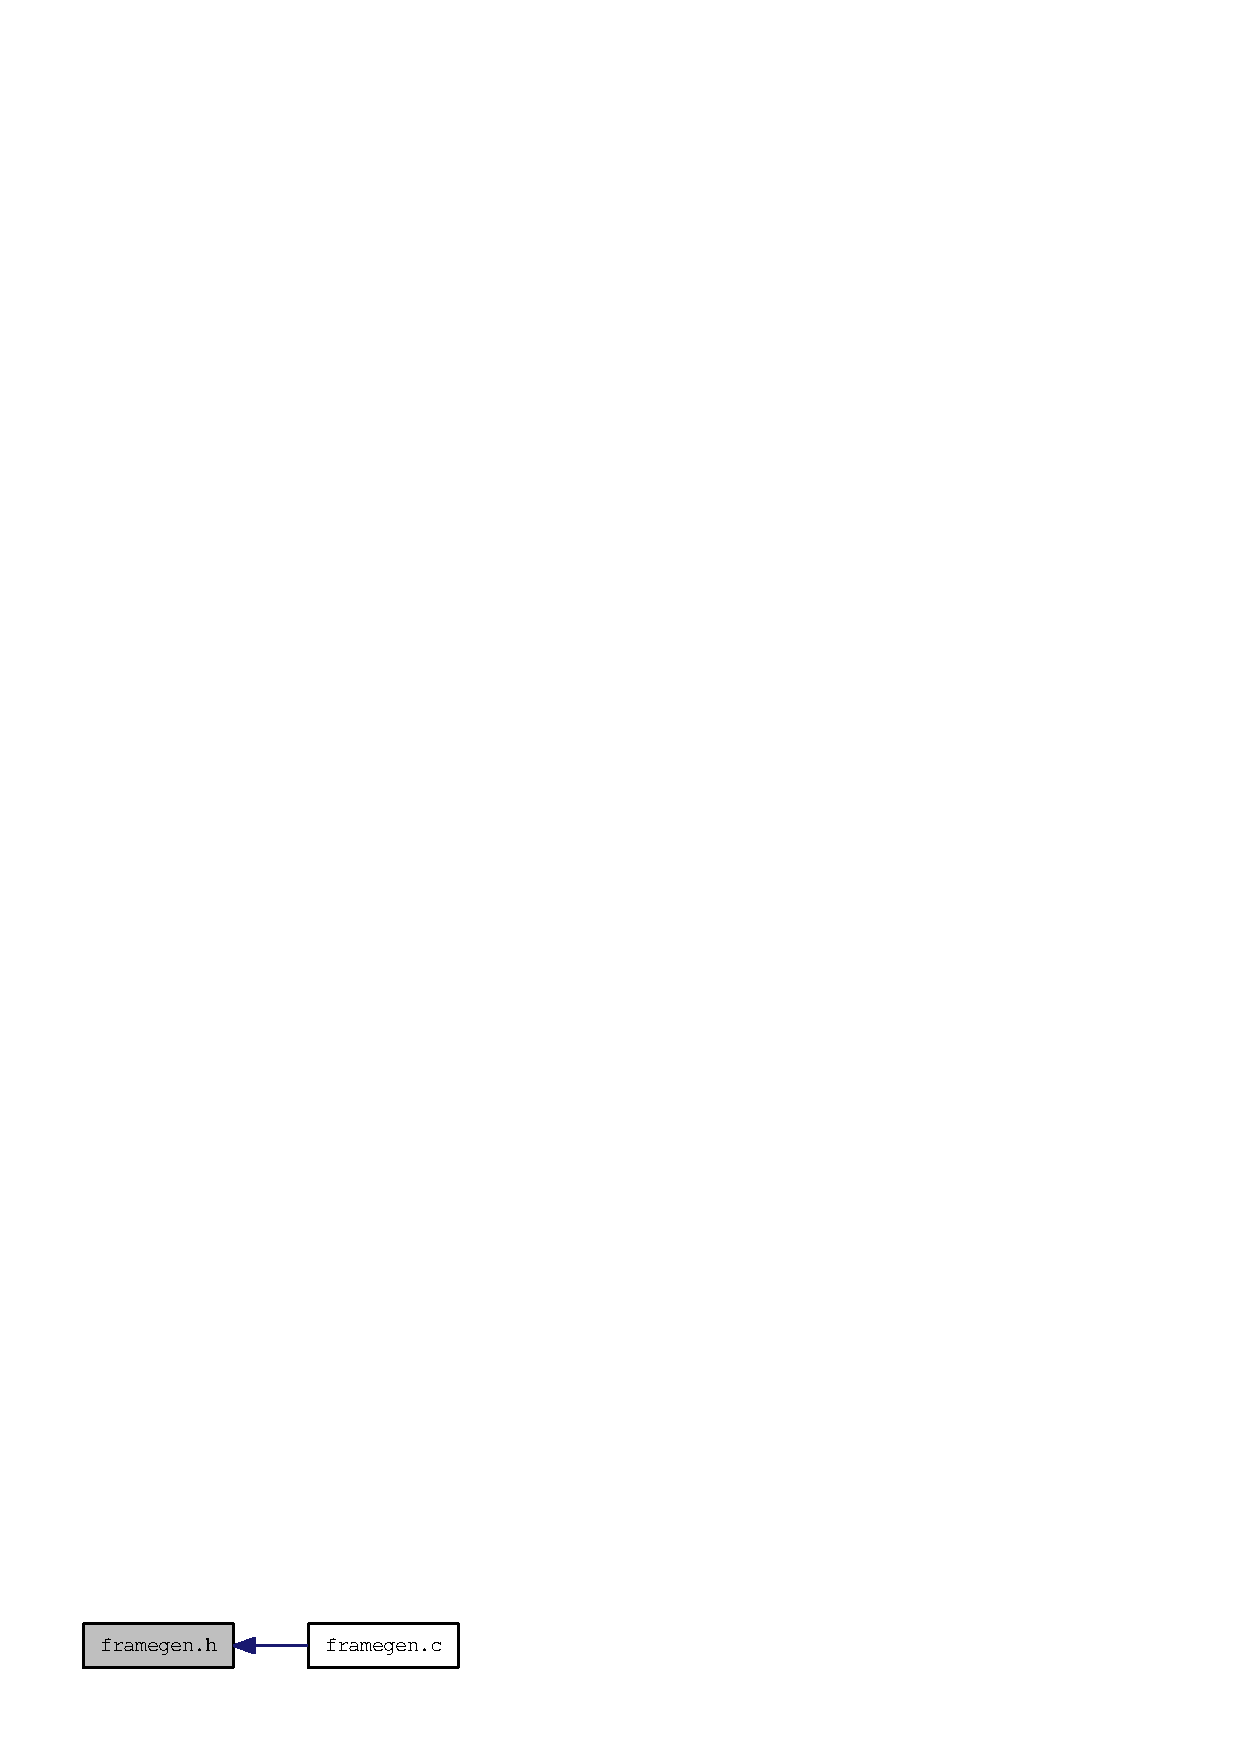
\includegraphics[width=112pt]{framegen_8h__dep__incl}
\end{center}
\end{figure}
\subsection*{Functions}
\begin{CompactItemize}
\item 
int \hyperlink{framegen_8h_64470613eeeb13398e90523259a10d8b}{commit} ()
\begin{CompactList}\small\item\em executes a previously written command \item\end{CompactList}\end{CompactItemize}


\subsection{Detailed Description}
The framegenerator for Xilinx FPGA. 

\begin{Desc}
\item[Author:]Dominik Fehlker \end{Desc}
\begin{Desc}
\item[Date:]\end{Desc}


Definition in file \hyperlink{framegen_8h-source}{framegen.h}.

\subsection{Function Documentation}
\hypertarget{framegen_8h_64470613eeeb13398e90523259a10d8b}{
\index{framegen.h@{framegen.h}!commit@{commit}}
\index{commit@{commit}!framegen.h@{framegen.h}}
\subsubsection[commit]{\setlength{\rightskip}{0pt plus 5cm}int commit ()}}
\label{framegen_8h_64470613eeeb13398e90523259a10d8b}


executes a previously written command 

\begin{Desc}
\item[Returns:]the errorcode \end{Desc}


Definition at line 31 of file framegen.c.

References rcu\-Single\-Write().

Referenced by main().

Here is the call graph for this function:\begin{figure}[H]
\begin{center}
\leavevmode
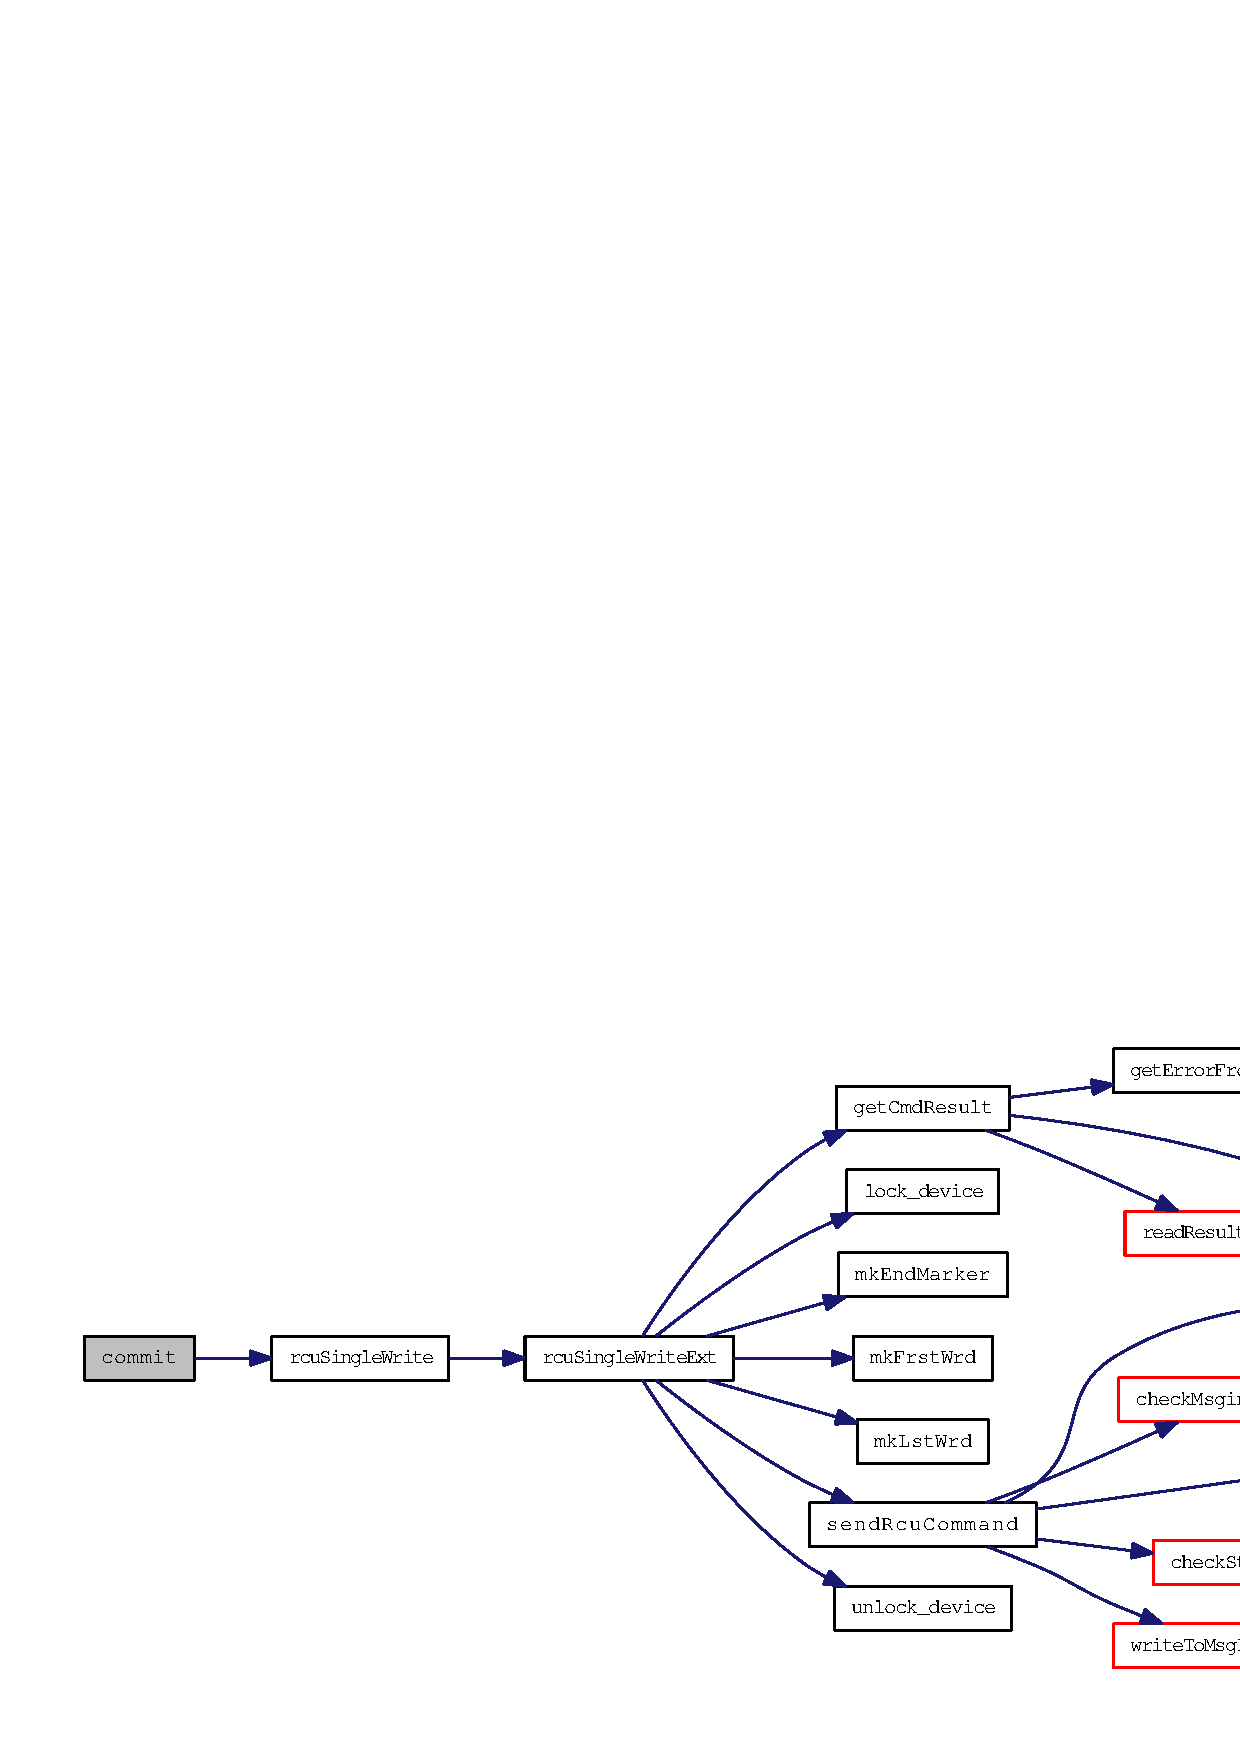
\includegraphics[width=394pt]{framegen_8h_64470613eeeb13398e90523259a10d8b_cgraph}
\end{center}
\end{figure}
